\chapter{Einführung}
\label{Einfuehrung}
Diese Ausarbeitung widmet sich dem \enquote{\ac{THB}} - also dem ausbalancieren von Bäumen bezüglich ihrer Höhe - als eine Form der durch Compiler durchgeführte Codeoptimierungen.

Hierbei wird zunächst eine Einordnung und Definition des \ac{THB} gegeben. Darauf aufbauend wird der in \cite{HeBIS-309344573} vorgeschlagene Algorithmus erläutert und aufgearbeitet. Auf Grundlage dieses Algorithmus wird ein Programm entwickelt, welches aus einem als Textdatei eingelesenen \ac{DG} Teilbäume extrahiert und auf diese \ac{THB} anwendet. Die konkrete Implementierung des Algorithmus wird zum Teil parallel erläutert - die komplette Implementierung (inklusive des Testprogramms) kann dem Anhang entnommen werden.

Abschließend wird ein Fazit gegeben.


\section{Einordnung in die Optimierungsverfahren}

Die Optimierungsverfahren, die ein Compiler anwendet, lassen sich primär danach kategorisieren, welchen Scope\footnote{dt.: Fokus, der Bereich des Programmcodes, welcher bei der Verarbeitung betrachtet wird.} sie auf den Code setzen. Dieser Scope reicht vom einzelnen Statement, bis zum kompletten Programmcode.

\begin{figure}[h]
	\centering
	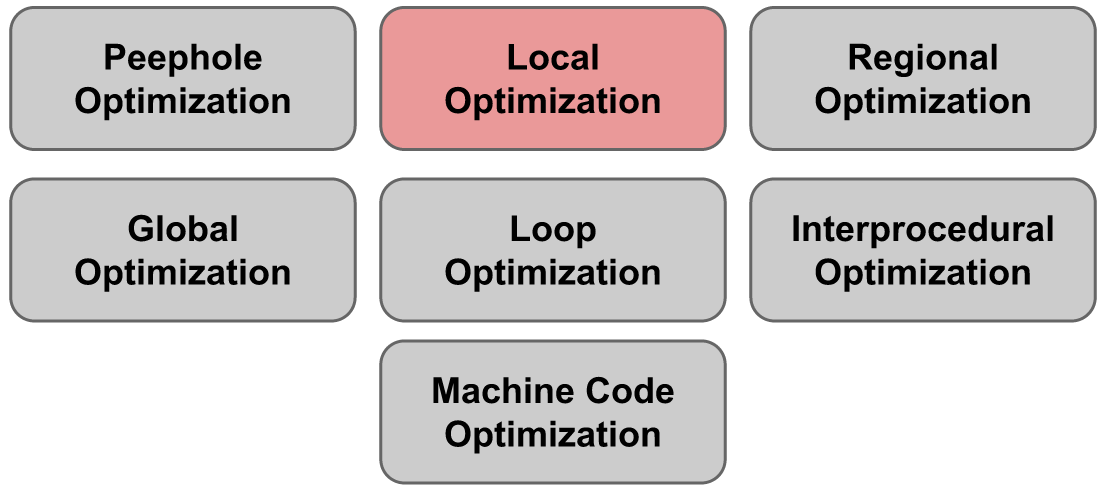
\includegraphics[scale=0.5]{images/Einordnung.png}
	\caption{Übersicht über Optimierungsverfahren.}
	\label{fig:Einordnung}
\end{figure}

Die in Abbildung \ref{Einfuehrung} zu sehenden Optimierungsverfahren lassen sich nun nach dem Scope kategorisieren. So arbeiten die \textit{Peephole Optimizations} und die \textit{Local Optimizations} auf den Basisblöcken. \textit{Regional Optimizations} und \textit{Loop Optimizations} setzen den Scope übergreifend auf mehrere Basisblöcke, wobei \textit{Global Optimizations} auf komplette Methoden angewendet werden. \textit{Interprocedural Optimizations} arbeiten gleichzeitig über mehrere Methoden und die \textit{Machine Code Optimizations} wird auf den fertigen Maschinencode angewendet.

Da \ac{THB} den Scope auf die Basisblöcke setzt, ist diese Technik - in Abbildung \ref{Einfuehrung} rot markiert - den lokalen Optimierungen zuzuordnen.

Ein Charakteristikum von Basisblöcken ist, dass es nur einen Einstiegspunkt sowie einen Ausstiegspunkt aus ebendiesen gibt. Daraus folgt, dass es innerhalb der Basisblöcke keinen Control-Flow gibt, wie es bei Methoden, Schleifen oder dem Programm in der Regel vorkommt - da die Basisblöcke die Knoten eines \ac{CFG} sind \cite{Allen:1970:CFA:390013.808479}. Hieraus lässt sich folgern, dass die Analyse, die bei der Optimierung vorgenommen werden muss, im Gegensatz zu anderen Verfahren relativ gering ist und ein großes Optimierungspotential besteht \cite{HeBIS-309344573}.




\section{Nutzen und Erwartungen}
\label{Nutzen}
Lineare Baumstrukturen entstehen oft durch lineare Blockabhängigkeiten. Diese Abhäng-igkeiten sind jedoch oft nicht zwingend linear. Beispiele hierfür finden sich beispielsweise in verschachtelten Strukturen von algebraischen Relationen.

Die Rechnung \ref{eq:beispiel-addition} wird oft mit einem rechts- oder links-assoziativen DG abgebildet. Dies führt dazu, dass in Mehrkernsystem die einzelnen Operationen nicht parallel durchgeführt werden können.

\begin{equation} \label{eq:beispiel-addition}
a + b + c + d + e + f + g + h
\end{equation}

In einer links-assoziativen Baumstruktur (siehe Abbildung \ref{fig:links-assoziativer-baum} \cite{HeBIS-309344573}) ist ein linearer Programmfluss vorgegeben. Jeder Schritt baut hierbei auf die vorherige Operation auf. In Tabelle \ref{tab:links-assoziativer-baum} \cite{HeBIS-309344573} sind die Befehle aufgelistet, welche aus dem links-assoziativen Baum in Abbildung \ref{fig:links-assoziativer-baum} folgen. Die Befehle sollen hierbei für einem 2-Kern-System optimiert werden. Die Bezeichner \textit{t1} bis \textit{t7} stehen dabei für die einzelnen Teilbäume, beziehungsweise die Zwischenergebnisse der Rechnung \ref{eq:beispiel-addition}. Wie zu sehen werden die Befehle nur auf einen Kern ausgeführt. Der andere Kern kann nicht agieren, da ihm immer eine Abhängigkeit zum Folgebefehl fehlt.

\begin{figure}
	\begin{center}
		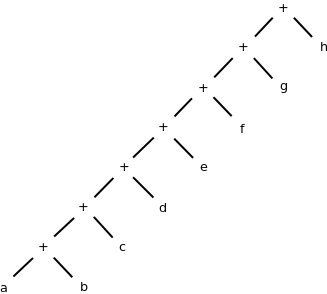
\includegraphics[width=0.5\textwidth]{images/links_assoziativer_baum}\\
	\end{center}
	\caption[Links-assoziativer Baum]{Links-assoziativer Baum (Vgl.: \cite{HeBIS-309344573})}
	\label{fig:links-assoziativer-baum}
\end{figure}

\begin{table}
	\begin{center}
		\begin{tabular}{|c|c|c|}
			\hline  & Kern 1 & Kern 2 \\ 
			\hline 1 & $ t1 \leftarrow a + b $& - \\ 
			\hline 2 & $ t2 \leftarrow t1 + c $& - \\ 
			\hline 3 & $ t3 \leftarrow t2 + d $& - \\ 
			\hline 4 & $ t4 \leftarrow t3 + e $& - \\ 
			\hline 5 & $ t5 \leftarrow t4 + f $& - \\ 
			\hline 6 & $ t6 \leftarrow t5 + g $& - \\ 
			\hline 7 & $ t7 \leftarrow t6 + h $& - \\ 
			\hline 
		\end{tabular}
	\end{center}
	\caption{Befehle für links-assoziativen Baum}
	\label{tab:links-assoziativer-baum}
\end{table}


Vorteilhaft wäre an dieser Stelle jedoch eine Codestruktur, welche auf Mehrkernsystemen (zum Teil) parallel ausgeführt werden kann. Dadurch könnten Prozessortakte und somit die Laufzeit des kompilierten Programmes eingespart werden.

Das Verfahren des \ac{THB} soll hierbei angewendet werden, um die links- oder rechts-assoziativen Bäume auszubalancieren. Sofern die Kinder eines Baumes nicht untereinander Abhängigkeiten aufweisen, können diese parallel vom Prozessor bearbeitet werden. Dies führt zur Ausführung vom mehreren Befehlen innerhalb eines Taktes in Mehrkernsystemen.

Außerdem soll das Ergebnis des \ac{THB} nicht über mehr Schritten bestehen, als die nicht balancierte Form. Sollte der optimierte Code auf einem Einkernsystem verwendet werden, darf es nicht mehr Zeit kosten, als der unoptimierte Code.


\section{Height-Balanced Tree}
Die Beschreibung \textit{\ac{HBT}} bezeichnet einen Binärbaum, dessen rechter und linker Unterbaum balanciert sind (s. Abbildung \ref{fig:vgl-hbt}) \cite{hbt}.


Um einen binären Baum als Height-Balanced zu erkennen, wird anhand von drei Punkten entschieden:

\begin{itemize} 
	\item Ein Baum ohne Unterbäume ist balanciert.
	\item Beide Unterbäume sind balanciert. 
	\item Die Differenz der maximalen Tiefen beider Unterbäume ist nicht großer als Eins. 
\end{itemize}

\begin{figure}
	\begin{center}
		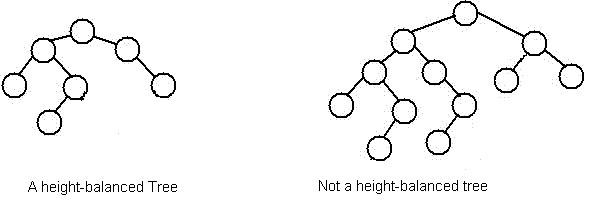
\includegraphics[width=0.8\textwidth]{images/balanced_tree}\\
	\end{center}
	\caption[Vergleich: Balancierter und unbalancierter Binärbaum]{Vergleich: Balancierter und unbalancierter Binärbaum \cite{geeks}}
	\label{fig:vgl-hbt}
\end{figure}


Diese Definition hilft im \ac{THB}, resultierende Bäume zu bewerten. Ist ein Baum nach Anwendung des \ac{THB} in Form eines \ac{HBT}, ist die Optimierung des Verfahrens bestmöglich durchgeführt worden.

Bezogen auf den links-assoziativen Baum aus Abbildung \ref{fig:links-assoziativer-baum} wäre ein \ac{HBT}-Äquivalent ein Baum, in dem das Addieren der Platzhalter (definiert durch a bis h) unabhängig von einander in Zwischenergebnissen passiert (s. Abbildung \ref{fig:balancierter-baum}).

\begin{figure}
	\begin{center}
		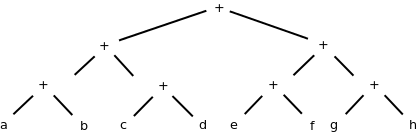
\includegraphics[width=0.5\textwidth]{images/balanced}
	\end{center}
	\caption[Balancierter Baum]{Balancierter Baum (Vgl.: \cite{HeBIS-309344573})}
	\label{fig:balancierter-baum}
\end{figure}

Die Codestruktur zu diesem Baum ist in Tabelle \ref{tab:balancierter-baum} zu sehen. Erkenntlich ist, dass mehrere Befehle gleichzeitig verarbeitet werden können, ohne dass diese aufeinander aufbauen bzw. warten müssen (z.B. \textit{t1} und \textit{t2}). Außerdem ist zu erkennen, dass im Vergleich zu Tabelle \ref{tab:links-assoziativer-baum} die Anzahl an Befehlen gleich geblieben ist. In einem Einkernsystem wäre die gebrauchte Zeit für diese Rechnung demnach gleich.

\begin{table}
	\begin{center}
		\begin{tabular}{|c|c|c|}
			\hline  & Kern 1 & Kern 2 \\ 
			\hline 1 & $ t1 \leftarrow a + b $ & $ t2 \leftarrow c + d $ \\ 
			\hline 2 & $ t3 \leftarrow e + f $ & $ t4 \leftarrow g + h $ \\ 
			\hline 3 & $ t5 \leftarrow t1 + t2 $ & $ t6 \leftarrow t3 + t4 $\\ 
			\hline 4 & $ t7 \leftarrow t5 + t6 $ &  -\\ 
			\hline 
		\end{tabular}
	\end{center}
	\caption{Befehle für balancierten Baum}
	\label{tab:balancierter-baum}
\end{table}